\section{Serverseitige Implementierung und Datenbank-Architektur}
Die serverseitige Implementierung bildet die Schnittstelle zwischen dem Client das heisst dem Internet Browser und den Messdaten. Diese müssen von den Sensoren in regelmässigen Abständen abgerufen und in der Datenbank gespeichert werden. Da die Datenbank das Herzstück der Wetterstation darstellt muss sie auch entsprechend geschützt werden vor Datenverlust und oder -manipulation. Die einzelnen Komponenten sowie der Aufbau der Datenbank werden im Folgenden erläutert.

%% ############################################################################
%% Unterkapitel
%% ############################################################################
\subsection{Datenerfassung}
Die einzelnen Daten werden unterschiedlich erfasst, wobei mit Ausnahme der Messwerten des Kombi-Wettertransmitters sämtliche Abfragen mittels Skripten durchgeführt werden. Ein Übersicht des Datenflusses ist in Abbildung\,\ref{img:datenerfassung} dargestellt. Im Folgenden werden die einzelnen Skripte erklärt.

\begin{figure}[htbp!]
  \fbox{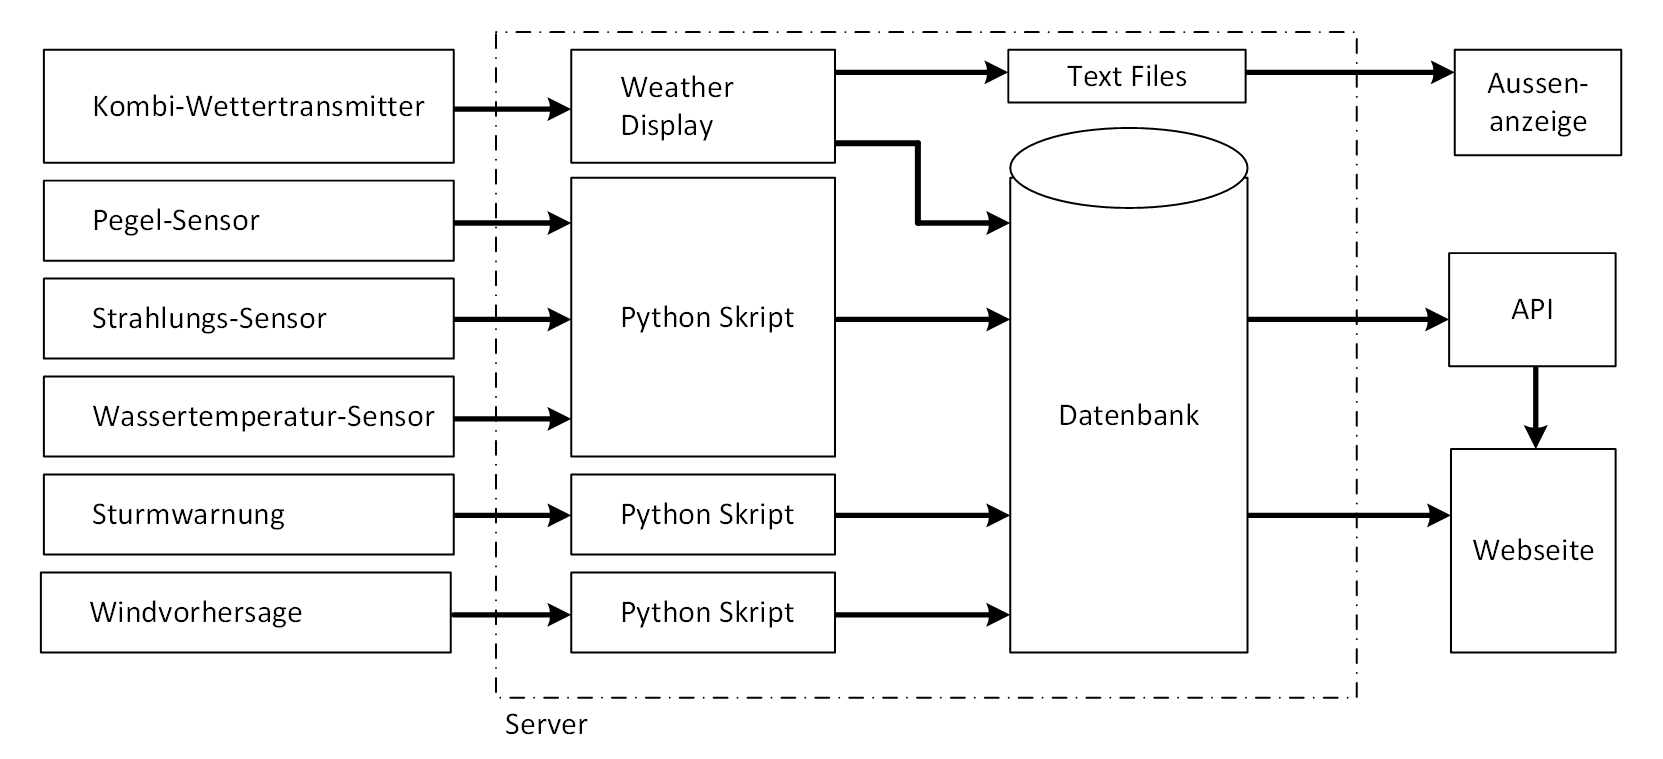
\includegraphics[width=\textwidth-2\fboxsep-2\fboxrule]{img/datenerfassung}}
	\centering
	\caption{Schematische Übersicht der Datenerfassung}
	\label{img:datenerfassung}
\end{figure}


\subsubsection{Erfassung der Messdaten des Kombi-Wettertransmitters}
Die Daten des Kombi-Wettertransmitters werden weiterhin von WeatherDisplay über eine virtuelle serielle Schnittstelle abgerufen, aufbereitet und im Minutentakt in die Datenbank gespeichert. Kann ein Datenbankeintrag aus irgendwelchen Gründen nicht erstellt werden, wird dies, wie später im Kapitel\,\ref{kap:Funktionsüberwachung} beschrieben, gemeldet. Weiter erzeugt Weather Display mehrere Text Files, welche unter anderem für die Aussenanzeige (Laufschrift am Hafengebäude) benötigt werden. Die Aussenanzeige ist aber nicht Bestandteil dieser Arbeit.

\subsubsection{Einlesen von Pegel-, Strahlungs-, und Wassertemperaturmesswerten}
Strahlungs- und Pegelsensor sind an einem Web-IO angeschlossen (siehe Datenblatt im Anhang\,\ref{Spec_webio}), welches die analogen Werte (in Milliampere) per Web-Schnittstelle zur Verfügung stellt. Die Abfrage erfolgt einmal pro Minute durch ein Python-Skript, wie in Listing \ref{lst:webIo} dargestellt. Die Temperatursensoren (PT100-Elemente) werden ähnlich erfasst mit dem Unterschied, dass nicht der Widerstandswert sondern direkt Grad Celsius geliefert wird. Als Schnittstelle wird an Stelle des Web-IO ein Web-Thermograph eingesetzt (siehe Datenblatt im Anhang\,\ref{Spec_webthermograph}).

\begin{lstlisting}[label=lst:webIo,caption=Python-Script zur Web-Abfrage des Pegel-Messwerts, language=python, style=py]
try:
    buffer = StringIO()
    c = pycurl.Curl()
    c.setopt(c.URL, 'http://webcam.wetter-arbon.ch:50506/single1')
    c.setopt(c.WRITEDATA, buffer)
    c.perform()
    c.close()
    requestMeasurement = buffer.getvalue()
\end{lstlisting}

\noindent
Der URL-Request wird mittels cURL ausgeführt. Die Abfrage ist für alle genannten Sensoren die gleiche, mit Ausnahme der Portnummer, welche sich je nach Sensor unterscheidet. Die Abfragen sind nach dem try... catch - Prinzip aufgebaut, sodass das Skript weiterläuft auch wenn ein Web-Interface nicht antwortet.



\subsubsection{Abgreifen der Sturmwarndaten} % screen scrapping
\label{kap:abgrSturmwarnung}
Die Sturmwarndaten werden periodisch mittels Python-Skript ausgelesen. Als Tool kommt die Python-Bibliothek \href{https://www.crummy.com/software/BeautifulSoup/}{\emph{BeautifulSoup}} zum Einsatz. Das Auslesen von Webseiten wird auch \emph{web scraping} genannt. Die Idee dahinter ist, die gewünschte Information auf Grund ihrer Element-Bezeichnung (z.B. \texttt{<td>}), ihres Attributs (z.B. \texttt{class="titelfett"}) oder Hierarchistufe (z.B. \texttt{tr:nth-of-type(4)}) eindeutig zu identifizieren. Um diese eindeutige Identifikation herauszufinden wurde das Google Chrome-Plugin \href{https://selectorgadget.com/}{\emph{SelectorGadget }} verwendet. Listing \ref{lst:kttgCrawler} zeigt die gesamte Abfrage. Darin ist auch das Problem dieser Methode gut erkennbar. Ändert die URL oder die Bezeichnung bzw. Struktur der Seite, liefert das Skript nicht mehr die gewünschten Daten. Da aber das Web-Scrapping die einzige kostenlose Möglichkeit darstellt um die Daten zu erhalten, muss dieses Risiko akzeptiert werden.


\begin{lstlisting}[label=lst:kttgCrawler,caption=Web-Scrapper für die Sturmwarndaten, language=python, style=py]
page = requests.get('http://www.kttg.ch/kapo/htm/stwarn.shtml')
soup = BeautifulSoup(page.text, 'html.parser')
# Einschaltzeit auslesen
soup.select('table tr:nth-of-type(4) td'):
# Status auslesen
soup.select('.titelfett strong'):
\end{lstlisting}


\subsubsection{Windvorhersagedaten}
Die Windvorhersagedaten von Windfinder werden ebenfalls mittels BeautifulSoup von der Webseite abgegriffen, analog der Sturmwarndaten in Kapitel\,\ref{kap:abgrSturmwarnung}. Beim Speichern der Vorhersagedaten in der Datenbank ist jedoch speziell, dass der angezeigte Wert erst in drei Tagen gilt. Umgekehrt heisst das, dass wenn der Vorhersagewert für jetzt benötigt wird, muss in der Datenbank das Datum von vor drei Tagen eingesetzt werden.
Um die Datenbankabfrage trotzdem möglichst einfach zu gestalten wurde eine VIEW verwendet. Diese wird dynamisch bei Aufrufen erzeugt und enthält die gewünschten Vorschaudaten aber mit dem aktuellen Datum. Dies vereinfacht den Aufbau des Verlaufsdiagramms.


% Der SQL-Befehl für die Erzeugung der VIEW ist vereinfacht in Listing \ref{lst:viewForecast} aufgeführt.
%
% Primär gibt es zwei Bedingungen. Erstens sollen nur die Dreitagevorhersagewert verwendet werden und zweitens sollen die Vorhersagewerte verwendet werden, die am nächsten bei der aktuellen Zeit liegen. Da das Vorhersageintervall 3 Stunden beträgt ist die Vorhersage maximal 1.5 Stunden verschoben.
%
% %View erstellen
% \begin{lstlisting}[label=lst:viewForecast,caption=Erzeugung der VIEW für den Forecast-Vergleich, language=SQL, style=htmlcssjs]
% SELECT *
% FROM 'tblcompwindfinder'
% WHERE
% (datetime + interval 3 day) <= now() #heute vor drei Tagen
% AND
% abs(timediff(datetime,now())) <= 13000) #innerhalb +/- 1.5h
% ORDER BY datetime DESC
% LIMIT 3
% \end{lstlisting}


%% ############################################################################
%% Unterkapitel
%% ############################################################################
\subsection{Datenspeicherung}
Für die Datenspeicherung stellt Hostpoint, der Webhosting-Provider der Wetterstation, eine Datenbank des Typs MariaDB Version 10.1 mit dem Administrationstool phpMyAdmin zur Verfügung. MariaDB ist eine relationales Open-Source-Datenbankverwaltungssystem und basiert auf MySQL. Die Datenbank der Wetterstation wurde komplett neu aufgebaut. Im Folgenden werde die einzelnen Tabellen und deren Struktur erklärt.

%Für die Umstrukturierung wurde von der Methodik aus dem Artikel Grundlagen und Entwurf \cite{Datenbanken:GrundlagenUndEntwurf:VeikkoKrypczyk} gebrauch gemacht.
%Wie in Introduction to relational Databases \cite{IntroductionToRelationalDatabases:MariaDB} beschrieben wird,

\subsubsection{Aufbau und Inhalt der Datenbank}
Die Datenbank besteht aus mehreren Tabellen mit unterschiedlichem Inhalt. Die Auflistung sämtlicher Tabellen mit einer Beschreibung des Inhalts befindet sich in Tabelle\,\ref{table:dbtabellen}. Die obersten vier Tabellen werden zur Speicherung der Messwerte/Zusatzinformationen verwendet. Anschliessend kommen die drei Tabellen für die historischen Daten und zum Schluss zwei Tabelle, die für den Benachrichtungsservice und die Webcam benötigt werden.
%\Diskussionspunkt{Warum wurde keine zweite DB für Benachrichtigungsservice und Webcam erstellt? Zweite DB mit igwetter_Services?}

% Datenbank-Tabellen
\begin{table}[htbp!]
  \setlength\extrarowheight{3pt} % for a more "open" look
  \begin{tabularx}{\textwidth}{|>{\RaggedRight\hspace{0pt}}p{4.5cm}|X|}

  \hline
  %\textbf{Tabelle}
  & \bfseries Beschreibung \\

  \hline
  \textbf{tblwettertransmitter}
  & Messwerte des Kombi-Wettertransmitters \\

  \hline
  \textbf{tblextsensors}
  & Messwerte der Sensoren (Bsp. Pegel) \\

  \hline
  \textbf{tblmisc}
  & Daten von Dritten (Bsp. Sturmwarnung) \\

  \hline
  \textbf{tblcompwindfinder}
  & Windvorhersagewerte von Windfinder \\

  \hline
  \hline
  \textbf{tbldatemaster}
  & Datumswerte von 2015 bis 2030 im Minutenabstand \\

  \hline
  \textbf{tblhistorical}
  & Messwerte zusammengefasst (1 Eintrag pro Stunde) \\

  \hline
  \textbf{tblwaterlevelhistorical}
  & Pegelwerte von 1953 bis heute (1 Eintrag pro Tag)\\

  \hline
  \hline
  \textbf{tblnotifications}
  & Abos des Benachrichtigungsservices \\

  \hline
  \hline
  \textbf{tblqueue}
  & Warteschlange der Webcam \\

  \hline
  \end{tabularx}
  \caption{Datenbanktabellen und deren Inhalt}
  \label{table:dbtabellen} % label muss NACH caption stehen!!!!
\end{table}

\noindent
Die Tabellen haben untereinander keine Verknüpfung (Relation), sondern sind alle eigenständig. Das einzige, was sie verbindet ist der Zeitstempel des Messzeitpunkts. Es wird deshalb auf die Erstellung eines ER-Modells, wie in Datenbanken Grundlagen und Design \cite{FrankGeisler2011mitpu} beschrieben, verzichtet. In Abbildung\,\ref{img:tabellenstruktur} ist beispielhaft die Struktur der Tabelle \emph{tblextsensors} aufgeführt. Als Primärschlüssel wird jeweils der Zeitstempel des Messzeitpunkts verwendet. Da der Primärschlüssel ein UNIQUE-Wert ist, wird verhindert, dass es zwei Einträge mit dem selben Zeitstempel gibt. Das komplette relationale Datenmodell mit allen Entitäten und deren Attributen befindet sich in Anhang\,\ref{anhang:relationalesDatenbankmodell}.

\begin{figure}[htbp!]
  \fbox{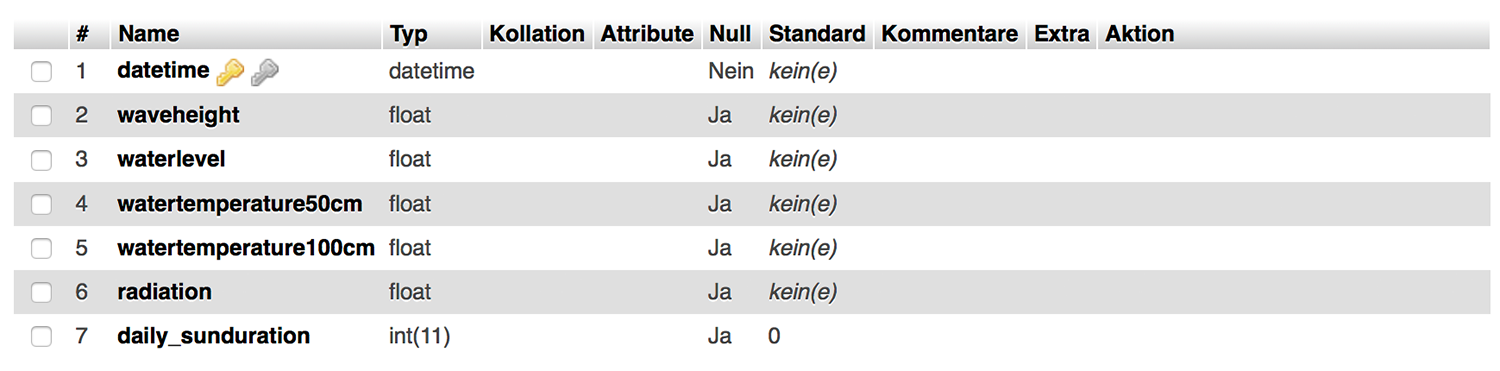
\includegraphics[width=\textwidth-2\fboxsep-2\fboxrule]{img/tabellenstruktur}}
	\centering
	\caption{Struktur der Tabelle \emph{tblextsensors}}
	\label{img:tabellenstruktur}
\end{figure}

%Die Normalisierung ist, wie in Datenbanken Grundlagen und Design \cite{FrankGeisler2011mitpu}, ein Prozess mit deren Hilfe die Datenbankstruktur optimiert wird und hilft dabei Datenredundanzen zu vermeiden. Da bei der Datenbank nur das Datum redundant ist, ist eine Normalisierung nicht notwendig.
%Das relationale Datenmodell unterscheidet sich in der Struktur nicht bedeutend vom ER-Modell. Der Unterschied  ist, dass die Primärschlüssel und die Datentypen festgelegt werden. Die sogenannten Schlüssel sind im relationalen Datenmodell auch ein wichtiges Merkmal. Bei zukünftigen Datenbankeinträgen sind entscheidend die Schlüssel, so kann verhindert werden, dass für einen gewissen Zeitpunkt nochmals Datensätze geschrieben werden.
%Die drei konzipierten Tabellen konnten wie gewünscht umgesetzt werden. Der Code für die Umsetzung der Tabellen, kann aus dem Anhang \ref{anhang:Datenbankcode} entnommen werden.\\


\subsubsection{Aggregation der historischen Daten}
\label{kap:aggregation}
Bei der Wetterstation fallen pro Minute rund 40 Datenpunkte an, die gespeichert werden. Pro Jahr sind dies über 21 Millionen Datenpunkte. Damit die Anzeige der historischen Messwerte nicht so viele Daten laden muss, werden die Messdaten periodisch zusammengefasst.
\newline

% Tabelle mit Minutenwerten
% Tabelle mit Tageswerten
% Wie funktioniert das Zusammenfassen der Daten -> SQL-Befehle

% \paragraph{Konzept}
\noindent
Die minütlich gespeicherten Messdaten werden einmal pro Stunde zusammengefasst und in die Tabelle mit den historischen Werten \emph{tblhistorical} geschrieben. Für die Aggregation wird die Median-Funktion verwendet um den Einfluss von Messfehlern zu reduzieren. Einmal pro Tag werden zudam die Pegeldaten des gesamten Tags gemittelt und in die Tabelle \emph{tblwaterlevelhistorical} geschrieben, wie in Abbildung\,\ref{img:historical} dargestellt.

\begin{figure}[htbp!]
  \fbox{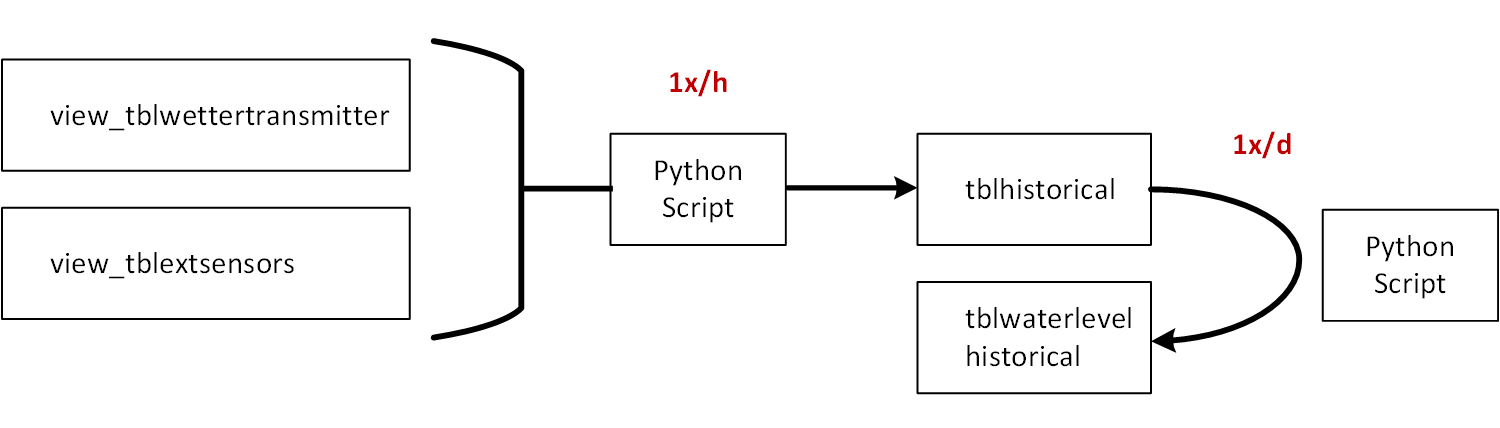
\includegraphics[width=\textwidth-2\fboxsep-2\fboxrule]{img/historical}}
	\centering
	\caption{Konzept der Datenaggregation}
	\label{img:historical}
\end{figure}


% \paragraph{LEFT JOIN}
Das Script, welches die minütlichen Daten zu Stundendaten aggregiert greift nicht direkt auf die Messwerttabellen zu, sondern auf sogenannte VIEWs. Eine VIEW ist eine virtuelle Tabelle. Sie enthält keine Daten, sondern verweist auf die zugrundeliegenden Basistabellen. VIEWs ermöglichen es komplexere Abfragen zu vereinfachen und mehrere Tabellen über JOIN-Verknüpfungen zu einer einzigen Tabelle zusammenzufassen.

\begin{figure}[htbp!]
  \fbox{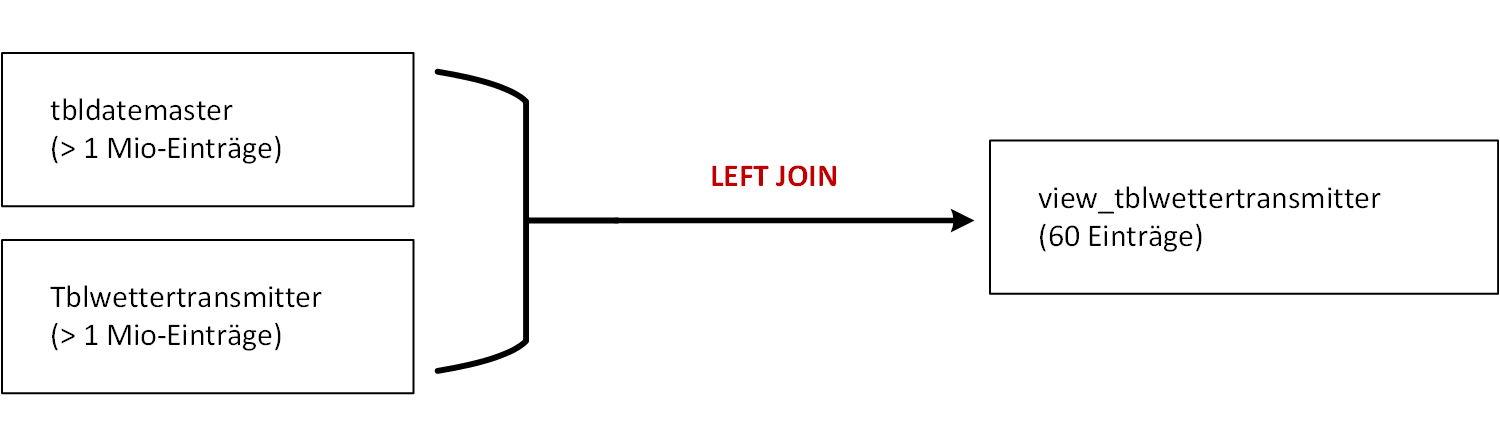
\includegraphics[width=\textwidth-2\fboxsep-2\fboxrule]{img/leftjoin}}
	\centering
	\caption{Konezpt der Datenaggregation}
	\label{img:leftjoin}
\end{figure}


Die beiden VIEWs, die für die Aggregation benötigt werden beinhalten jeweils genau 60 Einträge. Einen für jede Minute der vergangenen Stunde. Damit immer für jede Minute ein Eintrag vorhanden ist, auch wenn zum Beispiel der Sensor aus irgendeinem Grund keine Messwert geliefert hat, wurde ein LEFT JOIN mit der Datemaster-Tabelle erstellt. Diese Tabelle enthält sämtliche Datum/Zeit Einträge von 2015 bis 2035 im Minutenabstand.



%Bevor sich Gedanken um die Datensicherheit gemacht werden, sollten die Bedingungen an den Speicherplatz klar sein. Während der Laufzeit werden grosse Mengen an Daten in die Datenbank geschrieben. Vor der Neukonzipierung werden täglich 1440 Datensätze gespeichert. Das bedeutet jede Minute einen Datensatz. Ein Datensatz beinhaltet 65 Einträge, die gesamte relevante Datenbank igwetter wettertest benötigt (Stand 2018-04-24) 323.2  Mb. Die Tabelle wx data, beinhaltet die Minutenwerte des Wettertransmitters, benötigt davon (Stand 2018-04-24) 311.9 Mb, daraus erfolgt das ein Datensatz ca 0.025 Mb benötigt. Für den Speicherplatz, welcher 50 Gb bietet, stellt dies kein Problem dar. Hochrechnet reicht der Platz für die kommenden 45 Jahren.


% Die Herausforderung bei der Umsetzung war es, dass die historische Tabelle, welche aus den beiden Tabellen tblwettertransmitter und tblextsensors bestehen, mittels einer Query zusammenzubringen.

% Das Problem war die Zeit. Die Daten des Wettertransmitters werden Konfigurationsbedingt, nicht auf die Minute genau, sondern 31 Sekunden später geschrieben. Bei einem LEFT JOIN, welches über die Zeit geht, werden auch die Sekunden angeschaut. Nach mehreren gescheiterten Versuchen, ist es anschliessend gelungen, eine passende Query wie in \ref{lst:LeftJoinQuery} zu entwickeln.

% Zudem wird eine historische Tabelle erstellt, diese soll, die zu stündlich aufbereiteten Daten aus den beiden Tabellen enthalten.
% Um die historische Tabelle ohne Ausfälle zu füllen wird eine Tabelle entstehen, welche alle Zeitstempel von 2015 bis 2030 beinhaltet. Welche Datenpunkte übernommen werden, kann aus dem Anhang \ref{anhang:Datenbankschema} entnommen werden.\\

% Beim Modell der historischen Daten sieht das ganze anders aus (siehe Abb. \ref{img:ER_Modell historische Daten}). Hier beinhaltet jeder Zeitstempel, den Median, sowie die Extremwerte der Daten vom Wettertransmitter und die der externen Sensoren.

% Zusätzlich sollen die Daten, welche weiterhin im Minutentakt geschrieben werden, so aufbereitet werden, dass Benutzer auf der neu erstellen historischen Webpage die Wetterdaten der vergangenen Jahre einsehen können.


% \begin{lstlisting}[label=lst:LeftJoinQuery,caption=Json Struktur, language=JavaScript, style=htmlcssjs, mathescape]
% SELECT * FROM `DateMaster`
% LEFT JOIN `tblwettertransmitter`
% ON MINUTE(dt) = MINUTE(datetime)
% WHERE ((`DateMaster`.`dt` > (now() - interval 2 hour))
% AND((`tblwettertransmitter`.`datetime` > (now() - interval 2 hour))
% AND (hour((now() - interval 1 hour)) = hour(`tblwettertransmitter`.`datetime`)))
% AND (hour((now() - interval 1 hour)) = hour(`DateMaster`.`dt`))
% AND (`DateMaster`.`dt` < now()))
% order by `DateMaster`.`dt` desc
% \end{lstlisting} */


%\subsubsection{Zeitsynchronisation}
% welche Daten erhalten von wo einen Zeitstempel?
% woher erhalten diese Geräte die Zeit? Zeitserver?
%\Diskussionspunkt{Grafik einfügen}


\subsubsection{Datumsformatierung}
\label{kap:dateformat}
Die Norm DIN ISO 8601\footnote{DIN ISO 8601: Informationsaustausch - Darstellung von Datum und Uhrzeit} standardisiert die Darstellung von Datum und Zeit. Das internationale Datumsformat muss entweder als \texttt{2018-07-29T15:34:30} oder aber, wie empfohlen, mit der Differenz zur Koordinierten Weltzeit (UTC) \texttt{2018-07-29T15:34:30+02:00} angegeben werden. Bei der Wetterstation wird zwar das internationale Format verwendet, jedoch ohne ohne UTC-Angabe, da die Daten primär in der näheren Umgebung verwendet werden und somit direkt die lokale Zeit angezeigt wird.


\subsubsection{Umgang mit der Zeitumstellung}
Wie in Abschnitt\,\ref{kap:dateformat} erläutert, wird das Datum ohne Differenz zu koordinierten Weltzeit (UTC) gespeichert. Dies führt dazu, dass bei der Zeitumstellung im Frühling und im Herbst jeweils eine Stunde übersprungen beziehungsweise doppelt vorhanden ist. Damit das Vorgehen bei allen Datenbankeinträgen einheitlich ist, wurde das System von \emph{Weather Display} übernommen. Wird die Uhr vorgestellt so fehlt diese Stunde in der Datenbank (siehe Abbildung\,\ref{img:sommerzeit}) und beim Zurückstellen der Uhr wird die doppelte Stunde ignoriert. Da die Zeitumstellung in der Nacht stattfindet ist dieser Umstand für die Benutzer kaum bemerkbar.

\begin{figure}[htbp!]
  \fbox{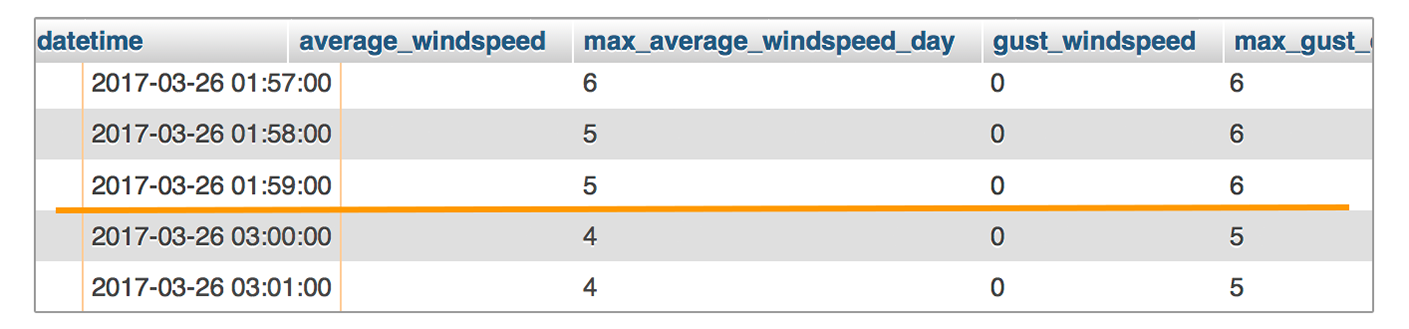
\includegraphics[width=\textwidth-2\fboxsep-2\fboxrule]{img/sommerzeit}}
	\centering
	\caption{Fehlende Stunde in der Datenbank bei der Zeitumstellung}
	\label{img:sommerzeit}
\end{figure}


%% ############################################################################
%% Unterkapitel
%% ############################################################################
\subsection{Automatisierung der repetitiven Aufgaben (Cronjobs)}

%wiederkehrende Aufgaben – sogenannte Cronjobs – zu automatisieren.
% Der Cron-Daemon dient der zeitbasierten Ausführung von Prozessen in Unix und unixartigen Betriebssystemen wie Linux

Die Wetterstation basiert auf vielen repetitiven Aufgaben wie zum Beispiel das minütliche Einlesen der Messdaten. Linux, welches auf dem Hostpoint-Server verwendet wird, bietet mit dem Cron-Daemon ein Werkzeug um zeitbasiert Befehle beziehungsweise Skripte (Cronjobs) auszuführen. Eine Liste sämtlicher Cronjobs, die die Wetterstation verwendet ist in Tabelle \ref{table:cronjobs} dargestellt. Um einen Cronjob zu definieren muss einerseits das auszuführende Skript angegeben werden und der Zeitpunkt, zu dem es ausgeführt werden soll. Es kann zwischen Minute, Stunde und Tag gewählt werden. Ein Stern (*) bedeutet zu jeder Minute/Stunde/Tag. Die historischen Daten (\emph{historical.py}) werden beispielsweise zu jeder Stunde jeweils um 5 Minuten nach zusammengefasst. Die Windvorhersage von Windfinder (\emph{forecastWindfinder.py}) werden alle drei Stunden abgefragt (02:37, 05:37 usw.). Die Cronjobs sind essentiell für die Funktion der Wetterstation, werden diese nicht durchgeführt, werden auch keinen Daten ausgelesen bzw. erstellt.

% Tabelle Cronjobs
\begin{table}[htbp!]
  \setlength\extrarowheight{3pt} % for a more "open" look
  \begin{tabularx}{\textwidth}{|X|>{\RaggedRight\hspace{0pt}}p{3.5cm}|X|>{\RaggedRight\hspace{0pt}}p{5.5cm}|}

  \hline
  %\textbf{Tabelle}
  \bfseries Minute
  & \bfseries Stunde
  & \bfseries Tag
  & \bfseries Befehl/Skript \\

  %\hline
  \hline
  37
  & 2,5,8,11,14,17,20,23
  & *
  &  forecastWindfinder.py \\


  \hline
  *
  & *
  & *
  & sturmwarnung.py \\

  \hline
  *
  & *
  & *
  & externSensors.py \\

  \hline
  *
  & *
  & *
  & notifications.py \\

  \hline
  5
  & *
  & *
  & historical.py \\

  \hline
  7
  & 0
  & *
  & historicalWaterlevel.py \\


  \hline
  \end{tabularx}
  \caption{Konfiguration der Cronjobs}
  \label{table:cronjobs} % label muss NACH caption stehen!!!!
\end{table}



%% ############################################################################
%% Unterkapitel
%% ############################################################################
\subsection{Datenbanksicherheit (Datenmanipulation und -verlust)}
Bei der Wetterstation Arbon sind keine persönlichen oder sicherheitsrelevanten Daten in der Datenbank gespeichert. Somit ist diese aus Sicht eines potentiellen Angriffes eher uninteressant. Dennoch sollten die Daten hinreichend geschützt sein, um einen Datenverlust beziehungsweise eine Datenmanipulation zu verhindern. Um dies zu erreichen werden mehrere Techniken eingesetzt, die im Folgenden beschrieben werden.

\subsubsection{Schutz vor SQL-Injection}
Laut den OWASP\footnote{OWASP: Open Web Application Security Project} Top 10, einer  \href{https://www.owasp.org/index.php/Category:OWASP_Top_Ten_Project}{Liste}, welche die wichtigsten Sicherheitsrisiken von Web-Applikationen aufzeigt, ist SQL-Injection seit Jahren auf Platz 1. SQL-Injection ist eine Methode eine Datenbankabfrage so zu manipulieren, dass der Angreifer Daten ausspähen oder verändern kann.

\vspace{3mm}
\begin{lstlisting}[label=lst:maskierung,caption=Anwendung der Prepared Statements (gekürzt), language=PHP, style=PHP]
// Insert-Befehl
$stmt = $dbh->prepare("INSERT INTO tbl (email) VALUES (:email)");
$stmt->bindParam(':email', $email);
$email = mysql_real_escape_ string($_GET['email']);
$stmt->execute();
$stmt->close();

// Select-Befehl
$stmt = $dbh->prepare("SELECT email FROM tbl WHERE email = ?");
$stmt->execute(array(mysql_real_escape_ string($_GET['email'])))
$stmt->fetch()
\end{lstlisting}
\vspace{3mm}

\noindent
Die API, welche als primäre Schnittstelle für das Auslesen der Daten verwendet wird, ist so aufgebaut, dass die Abfrage mittels \emph{White List Input Validation} durchgeführt wird. Das bedeutet, dass die eingegebene URL mittels \emph{switch case} mit allen möglichen gültigen Abfragen verglichen wird und dann entsprechend weiterbehandelt, wie in Listing\,\ref{lst:switchCase} auf Seite \pageref{lst:switchCase} dargestellt. Die Möglichkeit einer SQL-Injection ist auf diese Weise ausgeschlossen. Lediglich bei der Warteschlange der Webcam und beim Benachrichtigungsservice werden Daten direkt in die Datenbank geschrieben beziehungsweise daraus gelesen. In diesem Fall werden die SQL-Abfragen mittels \emph{Prepared Statements} durchgeführt und die Benutzereingaben \emph{escaped}, wie in Listing\,\ref{lst:maskierung} dargestellt.

% https://www.owasp.org/index.php/SQL_Injection_Prevention_Cheat_Sheet

\subsubsection{Einschränkung der Datenbankrechte}
Hostpoint bietet die Möglichkeit mehrere Datenbankbenutzer anzulegen. Diese können mit unterschiedlichen Rechten ausgestattet werden wie in Abbildung\,\ref{img:dbnutzer} ersichtlich.
Für die Datenbank wurden zwei Benutzer angelegt. \emph{igwetter\_Data} wird intern durch die Skripte verwendet um die Messdaten in die Datenbank zu speichern und hat entsprechend Schreibrecht. Der zweite Benutzer \emph{igwetter\_Tablea} hat nur Leserecht und wird zum Abrufen der Daten für die API und Tableau benötigt.

\begin{figure}[htbp!]
  \fbox{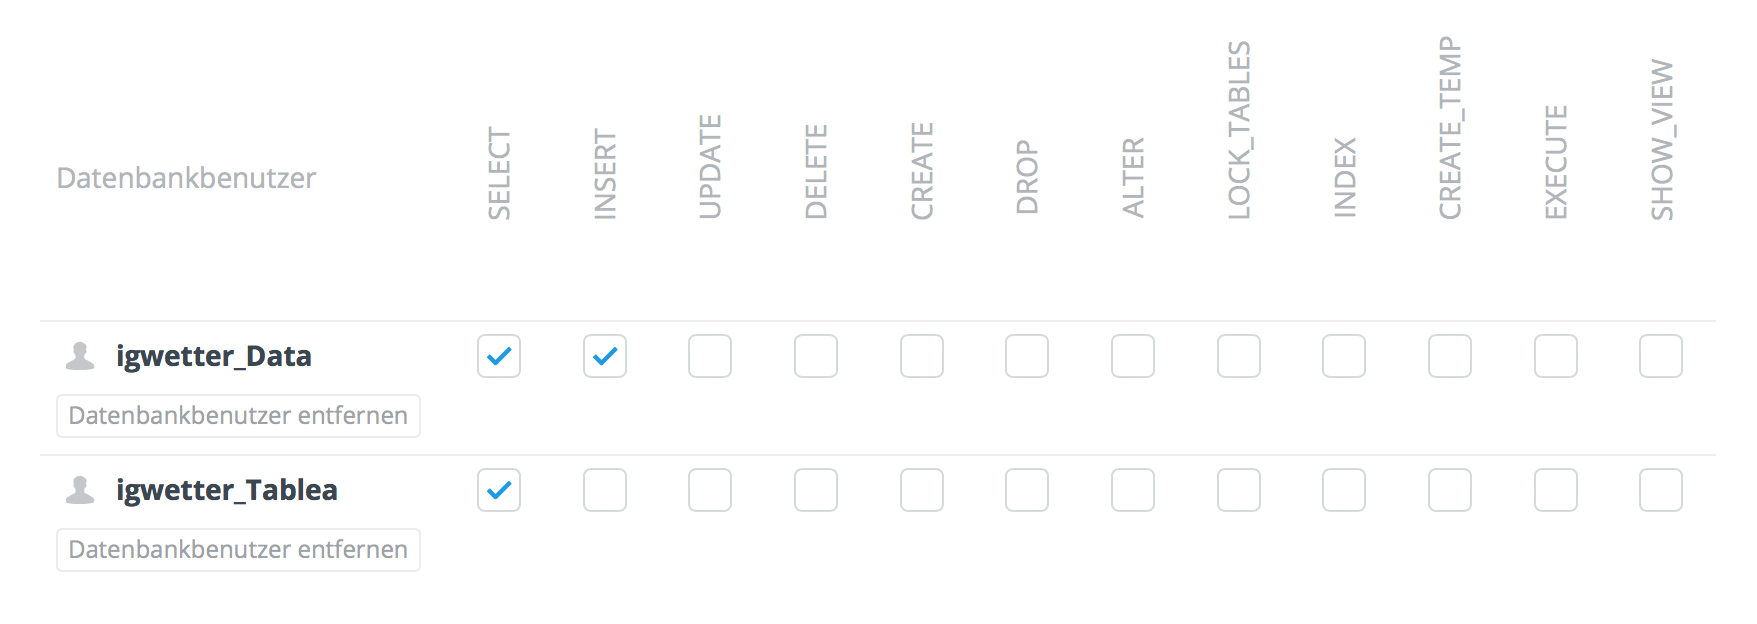
\includegraphics[width=\textwidth-2\fboxsep-2\fboxrule]{img/dbnutzer}}
	\centering
	\caption{Zuweisung der Rechte für unterschiedliche Datenbankbenutzer}
	\label{img:dbnutzer}
\end{figure}


\subsubsection{Backup}
Um die Datenbank gegen einen allfälligen Datenverlust zu sichern, ist ein regelmässiges Backup sinnvoll. Da die Wetterstation von einem Verein betrieben wird, ist der Aufwand auf ein Minimum zu reduzieren. Hostpoint bietet zwei Backup-Varianten an. Dies ist einerseits ein Backup mittels Cronjob auf zum Beispiel einen Cloud-Speicher und andererseits ein manuelles Backup auf eine externe Festplatte. Um den Aufwand klein zu halten, wird empfohlen ein monatliches Backup mit der manuellen Backup Funktion zu erstellen und dieses auf einer Festplatte zu speichern (siehe Abbildung \ref{img:backup}). Für Notfälle stellt Hostpoint zudem einen kostenpflichtigen Wiederherstellungs-Service zur Verfügung.

\begin{figure}[htbp!]
  \fbox{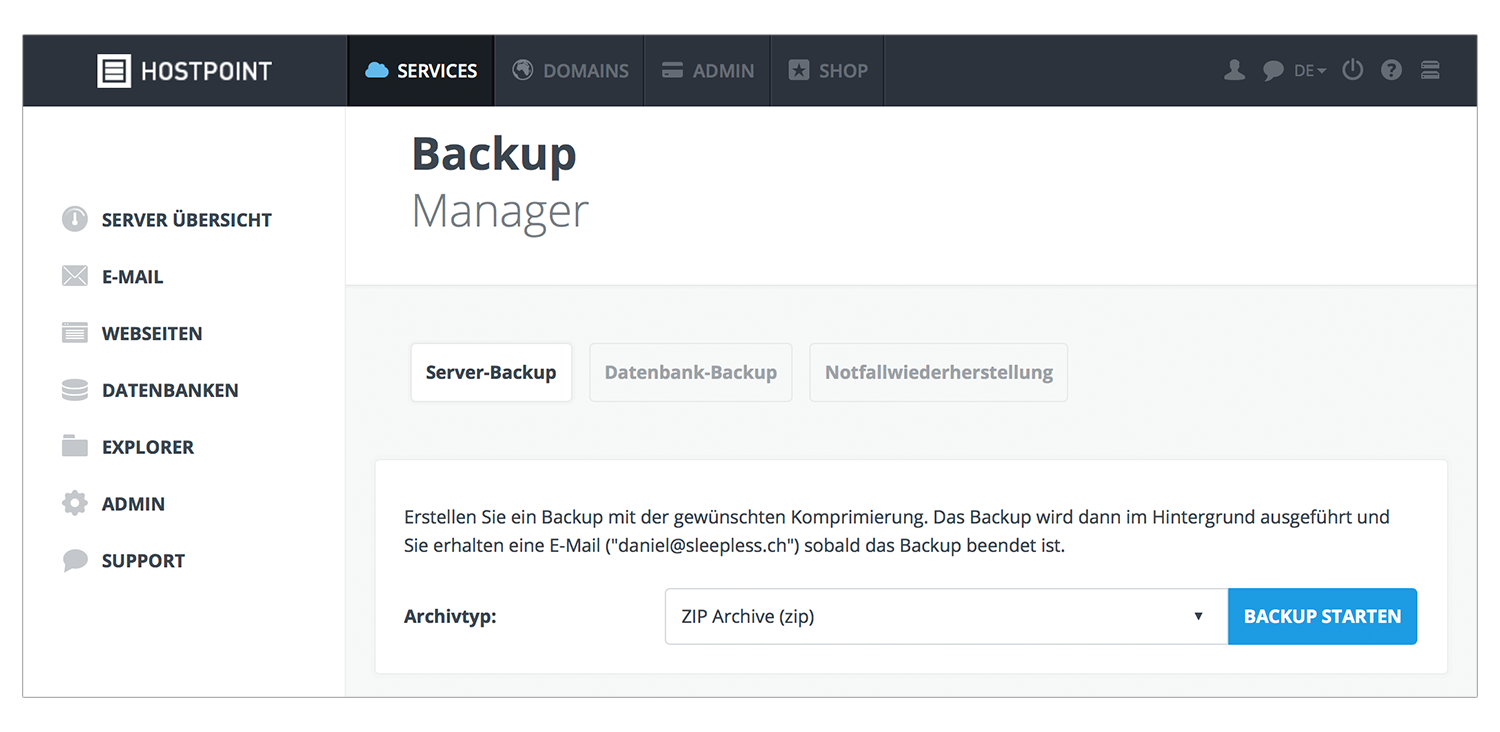
\includegraphics[width=\textwidth-2\fboxsep-2\fboxrule]{img/backup}}
	\centering
	\caption{Backup auf Knopfdruck von Hostpoint}
	\label{img:backup}
\end{figure}



%% ############################################################################
%% Unterkapitel
%% ############################################################################
\subsection{Funktionsüberwachung mittels Mail-Service}\label{kap:Funktionsüberwachung}
Die API und die Cronjobs laufen grundsätzlich selbständig. Trotzdem kann es vorkommen, dass eine Aufgabe nicht korrekt durchgeführt werden kann. Damit dies zeitnah bemerkt wird, wurde eine Funktionsüberwachung implementiert. Dies geschieht, indem sämtliche Aufgaben in den Python-Skripten in einem try...catch-Verfahren ausgeführt werden. Gibt es im try-Block ein Problem wird der Code unterbrochen und eine Exeption an den catch-Block übergeben. Anschliessend wird der Code nach dem Exception Handling ausgeführt\cite{ThePythonTutorial8.ErrorsAndExceptions:Python}. Folgende Aufgaben erzeugen bei einem Fehler eine Meldung:

\begin{itemize*}
\item Einlesen der Sensordaten (Wassertemperatur, Pegel, Strahlung)
\item Einlesen Wettertransmitter-Daten
\item Erstellung der stündlichen und täglichen historischen Daten
\item Einlesen der Sturmwarn- und Windprognosedaten
\item Benachrichtiungsservice
\end{itemize*}

\noindent
Die aufgezählten Funktionen werden alle bis auf das Einlesen der Wettertransmitter Daten über einen Cronjob ausgeführt. Hostpoint bietet die Möglichkeit, dass sämtliche Textausgaben (print-Funktion) eines Cronjobs an eine bestimmte Mailadresse gesendet werden (Listing \ref{lst:printfunction}). Der Service wurde so konfiguriert, dass er die Fehlermeldungen an die Mailadresse \emph{cronjob@wetter-arbon.ch} sendet. Der Posteingang kann dann an die entsprechenden Personen weitergeleitet werden. Kann zum Beispiel ein Messwert des Web-IO nicht abgerufen werden, wird eine Meldung wie in Listing\,\ref{lst:printfunction} erstellt.

\noindent
Da das Auslesen des Kombi-Wettertransmitters nicht mittels Cronjob durchgeführt wird gibt es die Möglichkeit des Exeption-Handlings nicht. Als Alternative wird aber beim Erstellen der historischen Daten kontrolliert, ob alle 60 Einträge der letzen Stunde vorhanden sind. Ist dies nicht der Fall, kann davon ausgegangen werden, dass Weather Display ein Problem hat.

\vspace{3mm}
\begin{lstlisting}[label=lst:printfunction,caption=Beispiel eines Exeption-Handlings, language=Python, style=py]
except Exception as e:
    print "Es ist ein Problem mit der Sonnenstrahlungs-Abfrage aufgetaucht: "
    print e
\end{lstlisting}
\vspace{3mm}


%% #########################################################################
%% Unterkapitel
%% ############################################################################
\subsection{Datenarchivierung und Speicherbedarf}
Pro Tag fallen bei der Wetterstation knapp 60'000 Datenpunkte an, die in der Datenbank gespeichert werden. Pro Jahr sind es über 21\,Millionen. Es stellte sich anfangs die Frage, ob die historischen Daten ausgedünnt werden sollen um Speicherplatz zu sparen. Stand Anfang August 2018, nach 3 Jahren Betrieb, waren jedoch nur 1.9\% der zur Verfügung stehenden 50\,GB belegt. Der Speicherplatz reicht somit, bei gleichbleibender Benützung, noch für die nächsten 50 Jahre. Es besteht somit keine Notwendigkeit die Daten auszudünnen d.h. es ist nicht vorgesehen irgendwelche Messdaten zu löschen. Die Zusammenfassung von Daten in die historische Datenbank wie in Kapitel\,\ref{kap:aggregation} beschrieben dient lediglich dazu die Performance der Anzeige der historischen Daten auf der Webseite zu verbessern.
